% Appendices A and B: single-column on new pages so that the timeline table and
% the multi-panel figures stay legible. Floats are pinned with [H] so each sits
% under its text. Tables in tables/ are generated from Phase1/results/summary/ by
% Phase1/harness/report_tables.py; figures come from Phase1/results/figures/.
\onecolumn
\raggedbottom
\setlength{\intextsep}{8pt plus 2pt minus 2pt}
\small

\section*{Appendix A: Timeline and Milestones}
Thanksgiving (Nov.~26--29) is treated as buffer.

\begin{center}
\begin{tabularx}{\textwidth}{@{}>{\raggedright\arraybackslash}p{1.6in}>{\raggedright\arraybackslash}X@{}}
\toprule
Stage & Work and milestones \\
\midrule
\textbf{1. Environment setup}\newline Nov 3--8 &
Confirm instance eligibility and vCPU quota; provisioning scripts; pinned
llama.cpp builds; GGUF and \texttt{mmproj} files on every device; WAN tunnel to
the laptops; per-device model agent; load generator and logging; pass-through
router. \textbf{M0 (Nov 4):} Phase~1 report. \textbf{M1 (Nov 8):} every device
serves 0.8B text and image requests through the router. \\
\addlinespace[3pt]
\textbf{2. Configuration testing and expectation setup}\newline Nov 6--18 &
E1--E5 sweeps over models, quantizations, lengths, image resolutions, load,
network, and model lifecycle; fit roofline efficiencies; collect tier labels;
freeze dev and held-out traces. \textbf{M2 (Nov 18):} calibrated cost model and
labeled dev set. \\
\addlinespace[3pt]
\textbf{3. Router development}\newline Nov 16--28 &
Baselines; ECT placement; R1--R2, then R3--R4; central-queue scheduler;
placement manager (stretch); decision-latency microbenchmarks.
\textbf{M3 (Nov 25):} router and baselines run end-to-end on dev mixes. \\
\addlinespace[3pt]
\textbf{4. Experiments and analysis}\newline Nov 25--Dec 10 &
Held-out runs across $\rho$ (steady and bursty; fastest device idle and busy);
ablations; repeated runs with confidence intervals; failure analysis; report
and artifacts. \textbf{M4 (Dec 5):} all runs complete. \textbf{M5 (Dec 10):}
final report. \\
\bottomrule
\end{tabularx}
\end{center}

\setcounter{figure}{0}
\setcounter{table}{0}
\renewcommand{\thefigure}{B\arabic{figure}}
\renewcommand{\thetable}{B\arabic{table}}
\section*{Appendix B: Phase 1 Measurements}
These are the first measurements, taken on one laptop endpoint (L in
Table~\ref{tab:endpoints}: Apple M4 Pro, 48\,GB unified memory) with Ollama
0.40.14 on the Metal GPU and thinking mode off; the AWS endpoints come next.
They cover isolated profiles and cold start (E1, E4) and answer quality (E5):
636 requests, all completed without failures or timeouts. The harness, raw
per-request logs, and the scripts that regenerate every table and figure below
are in the repository (\texttt{Phase1/run\_all.sh}). Two caveats apply
throughout. Quantization is not matched: Ollama's default Qwen3.5-0.8B and 2B
builds are MXFP8, while the other models are Q4\_K\_M. And
\texttt{qwen3-vl:4b}~($\dagger$) ignores the thinking-off flag in this Ollama
version, so hidden reasoning inflates its output; its numbers are reported but
not used in the conclusions.

\subsection*{B.1 Model profiles and cold start (E1, E4)}
Table~\ref{tab:e1} and Fig.~\ref{fig:e1} profile each model in isolation
(prompts of about 128--2,048 tokens, 3 repetitions per point, medians
reported). Decode speed tracks \emph{active} rather than total parameters: the
35B-A3B MoE decodes at 62\,tok/s, 70\% of the dense 2B's 88\,tok/s with
16$\times$ its parameters. Its costs show up elsewhere: prefill is about
3$\times$ slower than the 2B (719 vs.\ 2,110\,tok/s), it occupies 21\,GB, and a
cold start takes 9.1\,s instead of 0.6\,s. Image inputs add visual tokens that
grow with resolution (prompts grow from about 100 tokens at 256\,px to about
1,060 at 1024\,px), and TTFT grows 7--11$\times$ with them (Table~\ref{tab:img},
Fig.~\ref{fig:img});
every Qwen3.5 model named the tallest bar correctly at every resolution.

\begin{table}[H]
\centering
\caption{Per-model profile on the laptop endpoint: medians over warm text runs;
cold load time and resident memory from cold starts.}
\label{tab:e1}
\begin{tabular}{@{}lllrrrrr@{}}
\toprule
Model & Params & Quant. & Prefill (tok/s) & Decode (tok/s) & TPOT (ms) & Cold load (s) & Resident (GB) \\
\midrule
\texttt{qwen3.5:0.8b} & 0.85B & MXFP8 & 4,621 & 182 & 5.5 & 0.61 & 1.2 \\
\texttt{gemma3:1b} & 1.0B & Q4\_K\_M & 3,674 & 176 & 5.7 & 0.55 & 0.9 \\
\texttt{qwen3.5:2b} & 2.2B & MXFP8 & 2,110 & 88 & 11.3 & 0.61 & 2.9 \\
\texttt{qwen3-vl:4b}$^\dagger$ & 4.4B & Q4\_K\_M & 751 & 77 & 13.1 & 1.66 & 4.2 \\
\texttt{qwen3.5:35b} & 36B & Q4\_K\_M & 719 & 62 & 16.1 & 9.12 & 21.2 \\
\bottomrule
\end{tabular}

\end{table}

\begin{figure}[H]
\centering
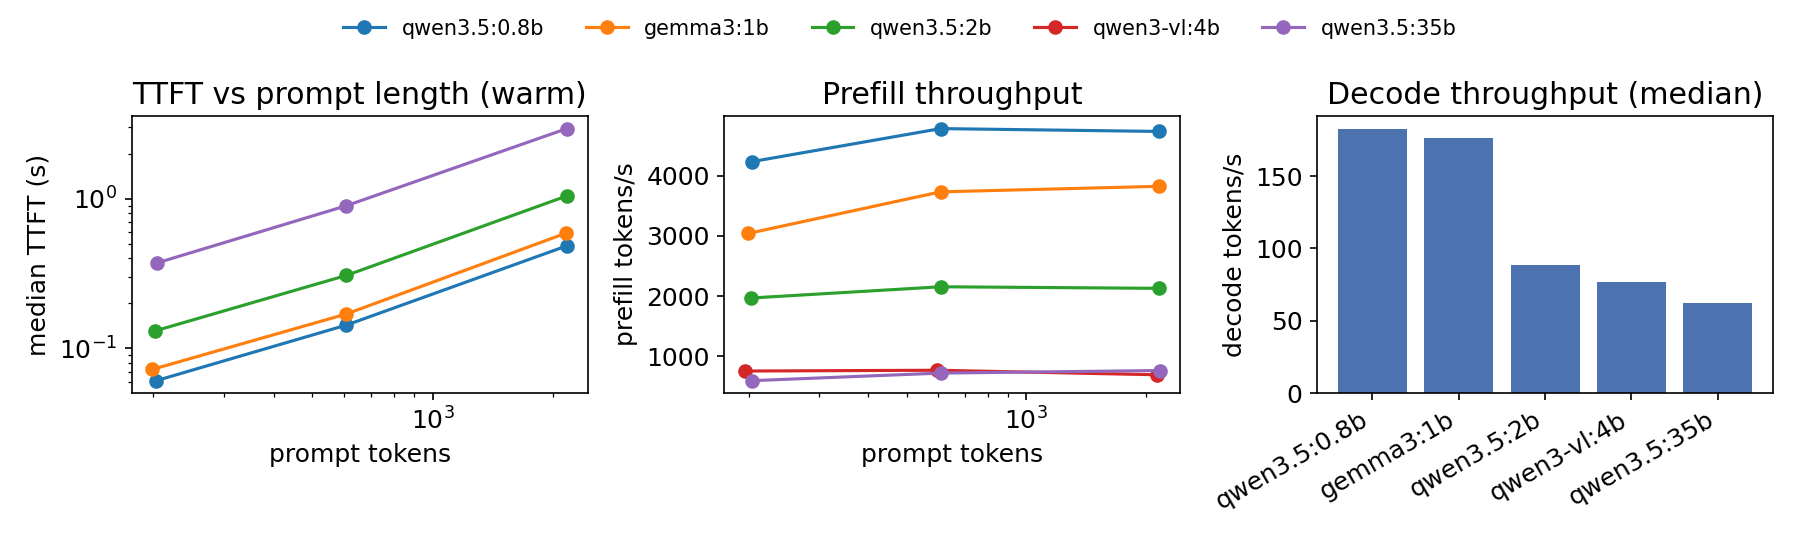
\includegraphics[width=\textwidth]{e1_profiles.png}
\caption{Isolated profiles (warm, medians of 3 runs). Left: TTFT vs.\ prompt
length. Middle: prefill throughput. Right: decode throughput.}
\label{fig:e1}
\end{figure}

\noindent\begin{minipage}[c]{0.47\textwidth}
\centering
\captionof{table}{Image requests: one bar chart and a question with a known
answer. Prompt tokens include the short text question.}
\label{tab:img}
\begin{tabular}{@{}rrrrr@{}}
\toprule
Image side & Prompt & \multicolumn{3}{c}{TTFT (s)} \\
\cmidrule(l){3-5}
(px) & tokens & 0.8B & 2B & 35B-A3B \\
\midrule
256 & 103 & 0.06 & 0.12 & 0.39 \\
512 & 294 & 0.13 & 0.30 & 0.80 \\
1024 & 1062 & 0.50 & 1.22 & 2.87 \\
\bottomrule
\end{tabular}

\end{minipage}\hfill
\begin{minipage}[c]{0.47\textwidth}
\centering
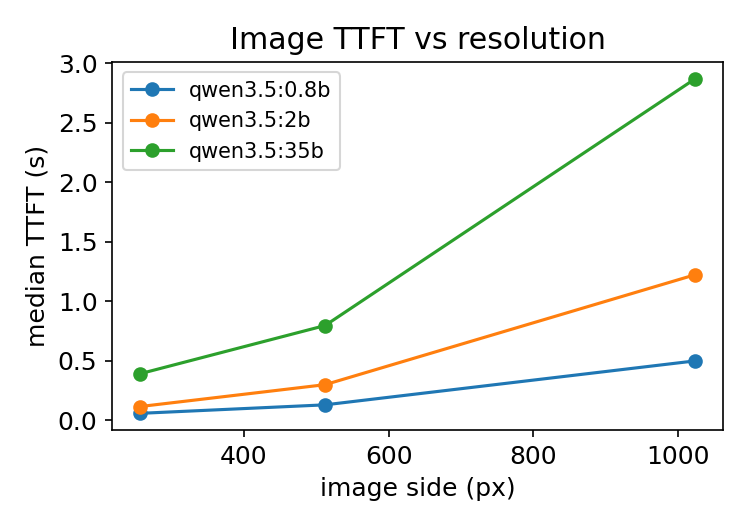
\includegraphics[width=\linewidth]{e1_image_ttft.png}
\captionof{figure}{Image TTFT vs.\ resolution (medians of 3 runs).}
\label{fig:img}
\end{minipage}

\subsection*{B.2 Answer quality and tier labels (E5)}
Every model answered the same 100 GSM8K test problems (temperature 0, at most
512 output tokens). Accuracy rises from 47\% for Qwen3.5-0.8B to 76\% for 2B
and 97\% for 35B-A3B (Table~\ref{tab:e5}, Fig.~\ref{fig:e5}). The last column
gives the tier labels: the smallest model that solves each problem. 47 problems
need only the 0.8B model, and just 11 need 35B-A3B.

\begin{table}[H]
\centering
\caption{GSM8K accuracy and tier labels (100 problems). \emph{Smallest correct
for}: number of problems for which this is the smallest model that answers
correctly.}
\label{tab:e5}
\begin{tabular}{@{}llrrrrr@{}}
\toprule
Model & Params & Accuracy & Output & \multicolumn{2}{c}{Latency (s)} & Smallest \\
\cmidrule(lr){5-6}
& & (\%) & tokens & mean & p95 & correct for \\
\midrule
\texttt{qwen3.5:0.8b} & 0.85B & 47 & 266 & 1.53 & 2.85 & 47 \\
\texttt{gemma3:1b} & 1.0B & 43 & 183 & 1.15 & 3.04 & 14 \\
\texttt{qwen3.5:2b} & 2.2B & 76 & 243 & 2.83 & 5.87 & 24 \\
\texttt{qwen3-vl:4b}$^\dagger$ & 4.4B & 44 & 461 & 8.75 & 10.41 & 2 \\
\texttt{qwen3.5:35b} & 36B & 97 & 160 & 3.11 & 5.69 & 11 \\
\midrule
\multicolumn{6}{@{}l}{No model correct} & 2 \\
\bottomrule
\end{tabular}

\end{table}

\begin{figure}[H]
\centering
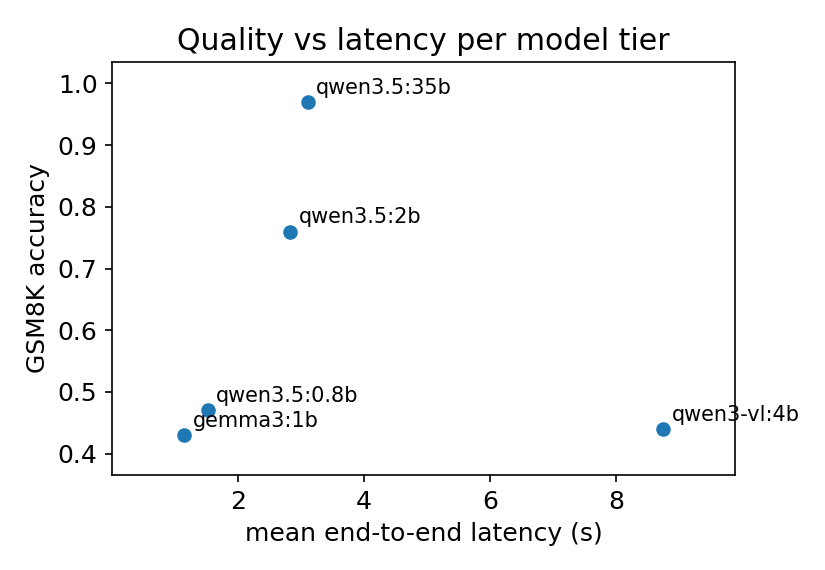
\includegraphics[width=0.5\textwidth]{e5_quality_latency.png}
\caption{GSM8K accuracy vs.\ mean end-to-end latency per model.}
\label{fig:e5}
\end{figure}

\newpage
\subsection*{B.3 Offline routing simulation}
Because every model answered every problem, a routing policy between a small
model and 35B-A3B can be scored exactly offline (Table~\ref{tab:route},
Fig.~\ref{fig:route}); latency is each model's measured single-request
latency, without queueing. A perfect router (oracle) between 0.8B and 35B-A3B
keeps 97\% accuracy and cuts mean latency by 18\% (3.11 to 2.54\,s). The R1
length rule reaches 91\% at 2.85\,s, while the R2 classifier, trained on only
100 labels with 5-fold cross-validation, barely separates easy from hard
problems. For the 2B pair the oracle saves only 9\%, because on this device the
MoE is nearly as fast as the dense 2B.

\begin{table}[H]
\centering
\caption{Offline routing between a small model and 35B-A3B on the E5 problems.
\emph{Latency}: mean single-request end-to-end latency. \emph{To 35B}: share
of problems sent to 35B-A3B.}
\label{tab:route}
\begin{tabular}{@{}lrrrrrr@{}}
\toprule
 & \multicolumn{3}{c}{0.8B $\rightarrow$ 35B-A3B} & \multicolumn{3}{c}{2B $\rightarrow$ 35B-A3B} \\
\cmidrule(lr){2-4}\cmidrule(l){5-7}
Policy & Acc.\ (\%) & Latency (s) & To 35B (\%) & Acc.\ (\%) & Latency (s) & To 35B (\%) \\
\midrule
Always the small model & 47 & 1.53 & 0 & 76 & 2.83 & 0 \\
Always 35B-A3B & 97 & 3.11 & 100 & 97 & 3.11 & 100 \\
Random (50/50) & 69 & 2.27 & 47 & 84 & 2.98 & 47 \\
R1 length rule: 35B-A3B if $>$31 words & 91 & 2.85 & 73 & 94 & 3.07 & 73 \\
R1 length rule: 35B-A3B if $>$39 words & 78 & 2.44 & 49 & 92 & 2.92 & 49 \\
R1 length rule: 35B-A3B if $>$49 words & 64 & 2.09 & 24 & 82 & 2.99 & 24 \\
R2 TF-IDF + logistic regression, $\tau=0.5$ & 89 & 2.88 & 85 & 76 & 2.83 & 0 \\
R2 TF-IDF + logistic regression, $\tau=0.7$ & 97 & 3.11 & 100 & 76 & 2.84 & 1 \\
Oracle (small when it is correct) & 97 & 2.54 & 53 & 98 & 2.84 & 24 \\
\bottomrule
\end{tabular}

\end{table}

\begin{figure}[H]
\centering
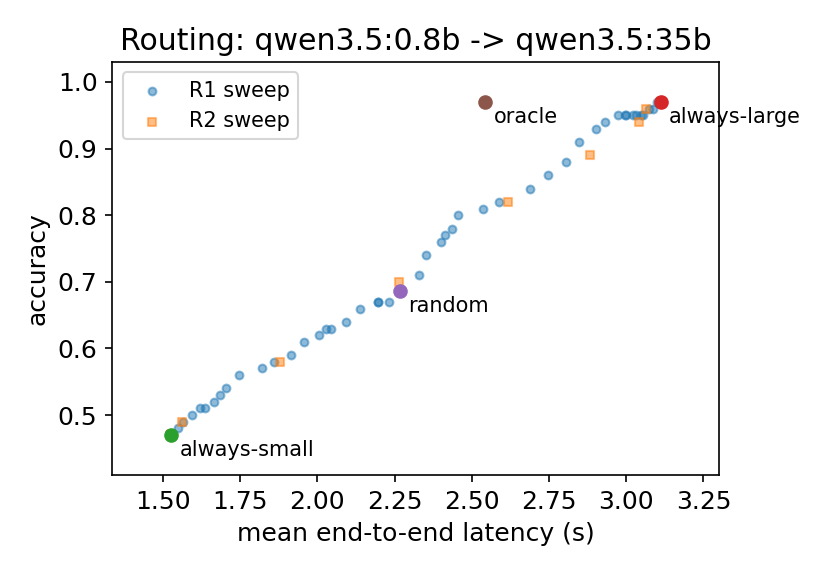
\includegraphics[width=0.48\textwidth]{route_sim_qwen3.5-0.8b__qwen3.5-35b.png}\hfill
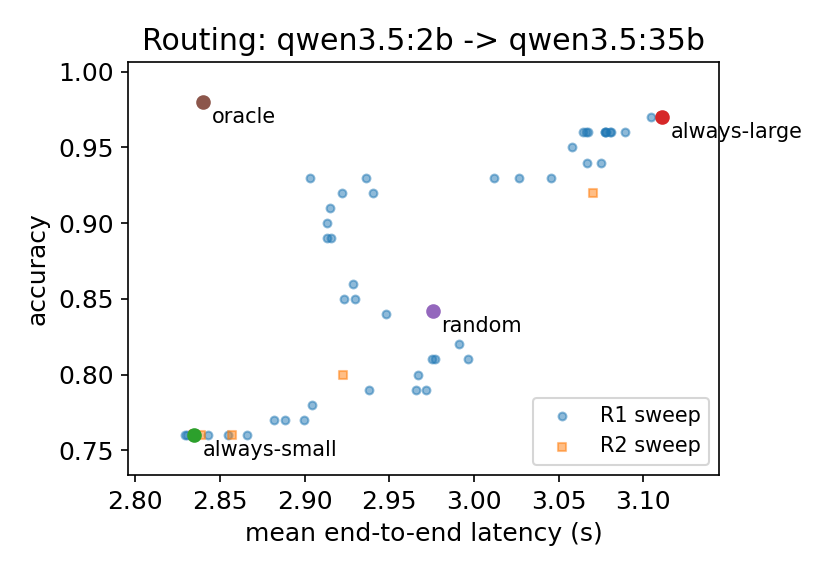
\includegraphics[width=0.48\textwidth]{route_sim_qwen3.5-2b__qwen3.5-35b.png}
\caption{Routing between a small model and 35B-A3B. Left: Qwen3.5-0.8B. Right:
Qwen3.5-2B. Small markers sweep the R1 length threshold and the R2 confidence
threshold $\tau$; labeled points mark the baselines and the oracle.}
\label{fig:route}
\end{figure}
